After establishing a theoretical foundation both about multigrid methods and evolutionary grammar-based optimization techniques, the first primary goal of this thesis is to develop a formal language for expressing arbitrarily structured multigrid solvers in a generalized way.
For this purpose, first observe that the multigrid solvers described Section~\ref{sec:multigrid-cycles} can be all classified by their \emph{cycle type}.
Each such cycle possesses a distinct computational pattern which stems from the number of recursive descents performed on each level of the method.
For instance a V-cycle is characterized by exactly one recursive descent per level.
All these classically considered multigrid cycles employ a fixed uniform number of recursive descents and smoothing steps per discretization level, which is determined by the parameters $\gamma$, $\nu_1$ and $\nu_2$ in Algorithm~\ref{alg:multigrid-cycle}.
While the representation of a multigrid method as a recursive cycle yields a formally simple and easily parameterizable algorithmic formulation it also enforces unnecessary restrictions on its structure.
Consider for instance the multigrid method depicted in Figure~\ref{fig:non-traditional-multigrid-cycle}.
\begin{figure}
	\begin{subfigure}{0.1\textwidth}
		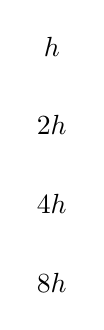
\begin{tikzpicture}
			\node   (h) at (-0.75, 4){$h$};
			\node   (2h) at (-0.75, 3){$2h$};
			\node   (4h) at (-0.75, 2){$4h$};
			\node   (8h) at (-0.75, 1){$8h$};
		\end{tikzpicture}
	\end{subfigure}
	\begin{subfigure}{0.9\textwidth}
		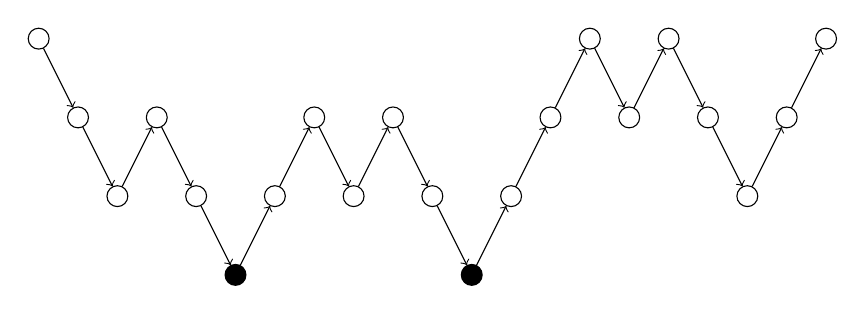
\begin{tikzpicture}
			\node	(a) at (0,4) [draw, circle,scale=0.8] {};
			\node	(b) at (0.5,3) [draw, circle,scale=0.8] {};
			\node	(c) at (1,2) [draw, circle,scale=0.8] {};
			\node	(d) at (1.5,3) [draw, circle, scale=0.8] {};
			\node	(e) at (2,2) [draw, circle, scale=0.8] {};
			\node	(f) at (2.5,1) [draw, circle,scale=0.8,fill=black] {};
			\node	(g) at (3,2) [draw, circle,scale=0.8] {};
			\node	(h) at (3.5,3) [draw, circle,scale=0.8] {};
			\node	(i) at (4,2) [draw, circle,scale=0.8] {};
			\node	(j) at (4.5,3) [draw, circle,scale=0.8] {};
			\node	(k) at (5,2) [draw, circle,scale=0.8] {};
			\node	(l) at (5.5,1) [draw, circle,scale=0.8,fill=black] {};
			\node	(m) at (6,2) [draw, circle,scale=0.8] {};
			\node	(n) at (6.5,3) [draw, circle,scale=0.8] {};
			\node	(o) at (7,4) [draw, circle,scale=0.8] {};
			\node	(p) at (7.5,3) [draw, circle,scale=0.8] {};
			\node	(q) at (8,4) [draw, circle,scale=0.8] {};
			\node	(r) at (8.5,3) [draw, circle,scale=0.8] {};
			\node	(s) at (9,2) [draw, circle,scale=0.8] {};
			\node	(t) at (9.5,3) [draw, circle,scale=0.8] {};
			\node	(u) at (10,4) [draw, circle,scale=0.8] {};
			\draw 
			(a) edge[->] (b) 
			(b) edge[->] (c)
			(c) edge[->] (d)
			(d) edge[->] (e)   
			(e) edge[->] (f)
			(f) edge[->] (g)
			(g) edge[->] (h)
			(h) edge[->] (i)
			(i) edge[->] (j)
			(j) edge[->] (k)
			(k) edge[->] (l)
			(l) edge[->] (m)
			(m) edge[->] (n)
			(n) edge[->] (o)
			(o) edge[->] (p)
			(p) edge[->] (q)
			(q) edge[->] (r)
			(r) edge[->] (s)
			(s) edge[->] (t)
			(t) edge[->] (u)
			;
		\end{tikzpicture}
	\end{subfigure}
	\caption{Example for a non-traditional multigrid method.}
	\label{fig:non-traditional-multigrid-cycle}
\end{figure}
While this method reaches the coarsest level twice and, hence, at first sight looks similar to a W-cycle, it employs a unique pattern of computations that is completely different from those of any of the traditional multigrid cycles.
As a consequence, this method can not be represented within the classical framework of multigrid cycles, as formulated in Algorithm~\ref{alg:multigrid-cycle}.
To overcome these limitations and construct multgrid methods with an arbitrary sequence of computations on each discretization level, as illustrated by the example in Figure~\ref{fig:non-traditional-multigrid-cycle}, a new formal language for their representation is needed.
The first step towards the development of this language is to find a way to represent the current state within each step of a multigrid method and then define transition rules between those states.
\section{Multigrid States}
\label{sec:multigrid-states}
In order to determine how the state of a multigrid method can be represented, we need to reconsider our original formulation of a multigrid cycle in Algorithm~\ref{alg:multigrid-cycle}.
The sake of simplicity, in the following we write symbols that correspond to vectors also in regular font.
In case the mathematical interpretation of a certain lower case symbol is ambiguous, its meaning will be explicitly stated. 
With the exception of the coarsest level, where the only allowed operation is the application of the coarse-grid solver, denoted by
\begin{equation*}
	x_{H} = A^{-1}_H b_H,
\end{equation*}
where $H$ is the discretization step size on the coarsest level, we can identify three elementary multigrid operations that can be employed within a cycle.
\begin{definition}[Elementary Multigrid Operations]
\label{def:elementary-multigrid-operations}
On each level $l > 0$ the following three operations are employed within a multgrid cycle.
\begin{itemize}
	\item \textbf{Smoothing}: Reduce the oscillatory error components of the approximate solution $\tilde{x}_h$ on the current level. 
	\begin{equation*}
		\tilde{x}_h = \tilde{x}_h + \omega M_h^{-1} \left( b_h - A_h \tilde{x}_h \right) \; \text{where} \; A_h = M_h + N_h
	\end{equation*}
	\item \textbf{Restriction}: Restrict the residual to obtain the right-hand side $b_{2h}$ of the error equation on the next coarser level.
	\begin{align*}
		\tilde{x}_{2h} & = 0 \\
		b_{2h} & = I_h^{2h} (b_h - A_h \tilde{x}_h)
	\end{align*}
	\item \textbf{Coarse-Grid Correction}: Prolongate a correction $\tilde{x}_{2h}$ obtained on a coarser grid to reduce the low-frequency error components of the approximate solution $\tilde{x}_h$.
	\begin{equation*}
		\tilde{x}_h = \tilde{x}_h + I_{2h}^h \tilde{x}_{2h}
	\end{equation*}
\end{itemize}
\end{definition}
Except for the operators $A_h$, $I_h^{2h}$ and $I_{2h}^h$ the result of each of these operations exclusively depends on the current value of the approximate solution on subsequent levels, i.e. $\tilde{x}_{h}$ and $\tilde{x}_{2h}$, and the right-hand side $b_h$.
However, in contrast to coarse-grid correction which utilizes the current approximate solution on the coarse grid, both smoothing and restriction first compute the residual $r_h = b_h - A_h \tilde{x}_h$, which can be considered as an intermediate step.
While this differentiation is not strictly necessary it leads to simpler operations, since both restriction and smoothing can then be split into two steps.
Furthermore, as in practice the actual error can usually not be computed, the residual is often the only available metric to investigate whether a multigrid iteration has achieved a certain amount of error reduction and, hence, has to be repeatedly computed.
%The residual is then either restricted and assigned to the right-hand side $b_{2h}$ or employed to reduce the oscillatory error components of the approximate solution by computing a correction term of the form $\omega A_h^{-1} r_h$.
To derive a general representation for the state of a multigrid method based on our previous observations, we consider the sequence of operations shown in Algorithm~\ref{alg:example-three-grid-method}, which corresponds to a three-grid V-cycle that performs one step of underrelaxed Jacobi smoothing on the second finest level.
\begin{algorithm}
	\begin{algorithmic}[1]
		\State $\tilde{x}_{h} = x_{h}^0$
		\State $r_{h} = b_{h} - A_h \tilde{x}_{h} $
		\State $ \tilde{x}_{2h} = 0$
		\State $ b_{2h} = I_{h}^{2h} r_{h}$
		\State $ r_{2h} = b_{2h} - A_{2h} \tilde{x}_{2h}$
		\State $ \tilde{x}_{2h} = \tilde{x}_{2h} + I_{4h}^{2h} A_{4h}^{-1} I_{2h}^{4h} r_{2h}$
		\State $ r_{2h} = b_{2h} - A_{2h} \tilde{x}_{2h}$
		\State $ \tilde{x}_{2h} = \tilde{x}_{2h} + 0.6 \cdot D_{2h}^{-1} r_{2h}$
		\State $\tilde{x}_{h} = \tilde{x}_{h}  + I_{2h}^h \tilde{x}_{2h}$
	\end{algorithmic}
\caption{Example for a three-grid V-cycle}
\label{alg:example-three-grid-method}
\end{algorithm}
In each step of this sequence of operations either the approximate solution, right-hand side or residual is updated on a certain level.
While in practice each of these variables corresponds to a data structure encompassing numerical values, our goal is to represent the algorithmic structure of a multigrid solver in the form of symbolic expressions.
In this case the value of each variable is determined by the expression that computes its value.
Updating a variable, therefore, corresponds to assigning a new expression to the corresponding symbol.
For this purpose, we consider the tuple
\begin{equation*}
	S_h = (\tilde{x}_h, b_h, r_h)
\end{equation*} 
on each level with step size $h$, which then contains expression of each of the corresponding three variables.
Starting from the first line we can then progressively update the contents of this tuple with the expression contained in each line, whereby the occurrence of each symbol is replaced by the respective expression currently contained in the tuple.
Figure~\ref{fig:example-tree-grid-method-states} shows the respective state tuple for each line of Algorithm~\ref{alg:example-three-grid-method}.
\begin{figure}
	\begin{equation*}
		\begin{array}{l l l}
			\hline
			\bm{S_h} & \bm{=} & \bm{(\tilde{x}_h, \, b_h, \, r_h)}  \\
			1: & &  x_{h}^0, \, b_h, \, \lambda \\
			2: & &  x_{h}^0, \, b_h, \, b_{h} - A_h x_{h}^0 \\ \hline
			\bm{S_{2h}} & \bm{=} &  \bm{(\tilde{x}_{2h}, \, b_{2h}, \, r_{2h})} \\
			3: & &  0, \, \lambda, \, \lambda \\
			4: & &  0, \, I_{h}^{2h}\underbrace{(b_{h} - A_h x_{h}^0)}_{r_{h}}, \, \lambda \\
			5: & &  0, \, I_{h}^{2h}(b_{h} - A_h x_{h}^0), \,\underbrace{I_{h}^{2h}(b_{h} - A_h x_{h}^0)}_{b_{2h}} - A_{2h} 0 \\
			6: & & 0 + I_{4h}^{2h} A_{4h}^{-1} I_{2h}^{4h} (\underbrace{I_{h}^{2h}(b_{h} - A_h x_{h}^0) - A_{2h} 0}_{r_{2h}}), \, I_{h}^{2h}(b_{h} - A_h x_{h}^0), \, \lambda\\
			7: & & 0 + I_{4h}^{2h} A_{4h}^{-1} I_{2h}^{4h} (I_{h}^{2h}(b_{h} - A_h x_{h}^0) - A_{2h} 0), \, I_{h}^{2h}(b_{h} - A_h x_{h}^0), \\ 
			& &  \underbrace{I_{h}^{2h}(b_{h} - A_h x_{h}^0)}_{b_{2h}} - A_{2h} (\underbrace{0 + I_{4h}^{2h} A_{4h}^{-1} I_{2h}^{4h} (I_{h}^{2h}(b_{h} - A_h x_{h}^0) - A_{2h} 0)}_{\tilde{u}_{2h}}) \\
			8: & &   (\underbrace{0 + I_{4h}^{2h} A_{4h}^{-1} I_{2h}^{4h} (I_{h}^{2h}(b_{h} - A_h x_{h}^0) - A_{2h} 0)}_{\tilde{u}_{2h}}) + 0.6 \cdot D_{2h}^{-1} \cdot \\ 
			& & (\underbrace{I_{h}^{2h}(b_{h} - A_h x_{h}^0) - A_{2h} (0 + I_{4h}^{2h} A_{4h}^{-1} I_{2h}^{4h} (I_{h}^{2h}(b_{h} - A_h x_{h}^0) - A_{2h} 0))}_{r_{2h}}), \\ 
			& & I_{h}^{2h}(b_{h} - A_h x_{h}^0), \, \lambda \\ \hline 
			\bm{S_h} & \bm{=} & \bm{(\tilde{x}_h, \, b_h, \, r_h)}  \\
			9: & & x_{h}^0 + I_{2h}^h ((0 + I_{4h}^{2h} A_{4h}^{-1} I_{2h}^{4h} (I_{h}^{2h}(b_{h} - A_h x_{h}^0) - A_{2h} 0)) + 0.6 \cdot D_{2h}^{-1} \cdot \\ 
			& &  (I_{h}^{2h}(b_{h} - A_h x_{h}^0) - A_{2h} (0 + I_{4h}^{2h} A_{4h}^{-1} I_{2h}^{4h} (I_{h}^{2h}(b_{h} - A_h x_{h}^0) - A_{2h} 0)))), \\ 
			& &  b_h, \, \lambda \\
			\hline
		\end{array}
	\end{equation*}
	\caption{State tuple in each step of Algorithm~\ref{alg:example-three-grid-method}.}
	\label{fig:example-tree-grid-method-states}
\end{figure}
As it has been introduced in Section~\ref{sec:formal-languages}, the empty symbol $\lambda$ denotes that a certain component of the tuple is unspecified.
After the last step of the sequence (line 9) the first component of the tuple ($\tilde{x}_h$) then combines all computational steps of the method in a single expression.

While Figure~\ref{fig:example-tree-grid-method-states} illustrates that the ternary tuple contains all relevant information of a multigrid method's current state on a certain level, we have not yet considered how to transition between the states of two subsequent levels.
First, consider the case of transitioning from a certain level with step size $h$ to the next coarser level with step size $2h$, which is shown in line 3 and 4 of Figure~\ref{fig:example-tree-grid-method-states}.
Here the tuple
\begin{equation*}
	S_{2h} = (0, \, I_{h}^{2h}(b_{h} - A_h x_{h}^0), \, \lambda)
\end{equation*} 
corresponds to the coarse-grid error equation 
\begin{equation*}
	A_{2h} x_{2h} = I_{h}^{2h}(b_{h} - A_h x_{h}^0),
\end{equation*}
whose solution is to be approximated starting with an initial guess of zero.
Therefore, all information to create this state is obtained from the next finer level in form of the restricted residual $I_h^{2h} r_h = I_h^{2h} (b_{h} - A_h x_{h}^0)$.
On the other hand, consider the transition from a coarse grid back to the next finer grid in form of the coarse-grid correction in line 9.
In this case we both require the approximate solution $\tilde{x}_{2h}$, computed on the coarse grid, as well as the previous values of the first two components $\tilde{x}_h$ and $b_h$ of the fine-grid state tuple.
While in the case of restriction we can neglect all previous states represented on the coarser grid, as it is explicitly contained in the residual, for a coarse-grid correction the previous state on the fine-grid needs to be restored.
Note that in case of a multigrid method that operates on a hierarchy of discretizations of even larger depth than the example shown in Algorithm~\ref{alg:example-three-grid-method}, this process must be recursively performed for each bottom up transition within the hierarchy.
To resolve this issue we need to extend our original formulation of a multgrid state by a fourth component with the purpose of preserving current state of the next finer level.
While at the topmost level this component is always empty, whenever restriction is performed the state of the current level is included.
For instance in line 4 of Figure~\ref{fig:example-tree-grid-method-states} we have to extend the given ternary tuple 
\begin{equation*}
S_{2h} = (0, \, I_{h}^{2h}(b_{h} - A_h x_{h}^0), \, \lambda)
\end{equation*}
by including the state 
\begin{equation*}
S_h = (x_{h}^0, \, b_h, \, b_{h} - A_h x_{h}^0, \, \lambda) 
\end{equation*} 
as an additional fourth entry. 
Hence, all required information for restoring the previous fine-grid state values is then included in the quaternary tuple 
\begin{equation*}
	S_{2h} = (0, \, I_{h}^{2h}(b_{h} - A_h x_{h}^0), \, \lambda, \, S_h).
\end{equation*}
%TODO clarify that line 3 and 4 can in practice be combined to one step
Note that since $S_h$ represents the current state on the finest grid, its fourth component is empty, while otherwise it would refer to the previous state of the next higher level in the discretization hierarchy.
To assess the feasibility of this approach, we have to check whether all components required to construct the coarse-grid correction expression, as in line 9 of Figure~\ref{fig:example-tree-grid-method-states}, are available within the current state.
However, since in addition to $\tilde{x}_{2h}$, both the approximate solution $\tilde{x}_h$ and right-hand side $b_h$ are now contained in the fourth component of the coarse-grid state tuple, this expression can be assembled in a straightforward manner.
At this point, it should be noted that coarse-grid correction from the coarsest grid represents a special case. 
Since the only allowed operation on this level is the application of the coarse-grid solver, which is denoted by a multiplication with the inverse of the system matrix, it is represented as a single operation in form of the expression 
\begin{equation*}
	\tilde{x}_{2h} = \tilde{x}_{2h} + I_{4h}^{2h} A_{4h}^{-1} I_{2h}^{4h} r_{2h}.
\end{equation*}
After resolving the issue of restoring previous states during coarse-grid correction, we can, thus, now provide a complete formal definition of the state of a multigrid method.
\begin{definition}[Multigrid State]
\label{def:multigrid-state}
The state of a multigrid method for solving the equation $A_{2h} x_{2h} = b_{2h}$ on a certain grid with step size $2h$ is given by the quaternary tuple
\begin{equation*}
	S_{h} = \left( \tilde{x}_{h}, b_{h}, c_{h}, S_{h/2}\right), 
\end{equation*}
where
\begin{itemize}
	\item $\tilde{x}_{h}$ is a mathematical expression for computing an approximate solution of the above equation,
	\item $b_{h}$ is an expression for computing the right-hand side of the above equation,
	\item $c_{h}$ is a correction term for improving the accuracy of the approximate solution,
	\item $S_{h/2}$ is either the current state on the next finer level with a step size $h/2$ or the empty symbol $\lambda$ in case $h$ represents the topmost level in the given hierarchy of discretizations.
\end{itemize}
\end{definition}
Note that in Definition~\ref{def:multigrid-state} the third component $c_{2h}$ of a multigrid state no longer only refers to the residual, but now represents an expression that corresponds to a general correction term.
While in the classical multigrid formulation, as presented in Section~\ref{sec:multigrid-methods}, all smoothing expressions are directly derived from the residual, alternative relaxation methods which can not be easily formulated in the simple framework of stationary iterative methods, such as distributive smoothing, have been proposed~\cite{trottenberg2000multigrid}.
Furthermore, the general notion of a correction term enables us to also represent intermediate expressions that do not specifically refer to the current residual within a multigrid state, for instance $c_h = \omega M_h^{-1} \left( b_h - A_h \tilde{x}_h \right)$ which corresponds to the complete term that is added to the current approximate solution within smoothing.   
%Finally, note that the computation of the coarse-grid correction does not require the value of the previous fine-grid residual.
%Therefore, the corresponding expression does not need to be restored and the residual can be omitted in the respective state tuple when performing the fine-to-coarse grid transition.
\section{State Transition Functions}
\label{sec:multigrid-state-transitions}
After defining the state of a multigrid method, the next step towards developing a formal language for representing arbitrary sequences of multigrid operations,
such as the one shown in Figure~\ref{fig:non-traditional-multigrid-cycle}, is to formally define a set of rules that describes the transitions between all possible states.
For this purpose, we need to consider the set of possible operations within a multigrid method, as shown in Definition~\ref{def:elementary-multigrid-operations}.
From a mathematical point of view, these operations exclusively consist of either matrix-vector multiplications or vector additions and subtractions.
First of all, the computation of the residual $r_h = b_h - A_h \tilde{x}_h$ represents the fundamental operation based on which an approximation to the solution of the target system $A_h x_h = b_h$ is iteratively improved, either with means of smoothing or by computing a coarse-grid correction.
The \textsc{residual} function implements the corresponding state transition for computing the residual on a certain level with step size $h$.
For this purpose first the residual expression is assembled based on the system matrix $A_h$ and the given state $S_h = (\tilde{x}_h, b_h, \lambda, S_{h/2})$, which contains the current approximate solution $\tilde{x}_h$ and right-hand side $b_h$.
The resulting expression is included as a the correction term $c_h$ into $S_h$, which is then returned at the end of the function.
\begin{algorithm}
	\begin{algorithmic}
		\Function{residual}{$A_h$, $(\tilde{x}_h, b_h, \lambda, S_{h/2})$}
		\State $c_h \gets b_h - A_h \tilde{x}_h$
		\State return $(\tilde{x}_h, b_h, c_h, S_{h/2})$
		\EndFunction
	\end{algorithmic}
\label{alg:state-transition-residual}
%\caption{Residual computation}
\end{algorithm}
After constructing an initial correction $c_h$ from the residual expression $b_h - A_h \tilde{x}_h$, next we can apply an operator $B_h$ to this term, either as part of a smoothing expression or in form of restriction to obtain the right-hand side $b_h$ of the coarse-grid error equation.
Since both operations can be formulated as a matrix-vector multiplication, we consider this operator application as an intermediate step that is implemented in form of the function \textsc{apply}.
This function applies to operator $B_h$ to the current correction term. 
The resulting expression then serves as a new correction term within the returned state.
\begin{algorithm}
	\begin{algorithmic}
		\Function{apply}{$B_h$, $(\tilde{x}_h, b_h, c_h, S_h)$}
		\State return $(\tilde{x}_h, b_h, B_h\cdot c_h, S_h)$
		\EndFunction
	\end{algorithmic}
\caption{Operator application}
\end{algorithm}
In general, the choice of the operator $B_h$ corresponds to the two elementary options available within a multigrid method, i.e. smoothing and solving the given problem on a coarser grid.
For instance, the choice of $B_h = D_h^{-1}$ leads to the expression
\begin{equation*}
	c_h = D_{-1} (b_h - A_h \tilde{x}_h),
\end{equation*}
which corresponds to one step of the Jacobi method as shown in Equation~\ref{eq:jacobi-method}.
In contrast, choosing $B_h$ as the restriction operator $I_h^{2h}$ leads to
\begin{equation*}
	c_{2h} = I_{h}^{2h} (b_h - A_h \tilde{x}_h),
\end{equation*}
which then serves as a right-hand side $b_{2h}$ of the corresponding coarse-grid error equation.
In both cases the correction term obtained from the \textsc{apply} function serves a different purpose.
First of all, we must be able to generate an expression that computes an improved approximate solution $\tilde{x}_h$ by applying an update in form of the correction term $c_h$ to the previous value of $\tilde{x}_h$. 
This behavior is implemented in the function \textsc{iterate}, which returns a state tuple with the expression for computing an updated approximate solution as its first entry.
\begin{algorithm}
	\begin{algorithmic}
		\Function{iterate}{$\omega$, $P$, ($\tilde{x}_h$, $b_h$, $c_h$, $S_{h/2}$)}
			\State $\tilde{x}_h \gets \tilde{x}_h + \omega \cdot c_h$ with $P$
			\State return ($\tilde{x}_h$, $b_h$, $\lambda$, $S_{h/2}$) 
		\EndFunction
	\end{algorithmic}
%\caption{Iteration}
\end{algorithm}
In addition to the mere application of a correction term, this function also includes a relaxation factor $\omega$ and partitioning operator $P$ which enables both the formulation of underrelaxed, overrelaxed and potentially colored versions of each operation, for instance those described in Section~\ref{sec:rb-gs}.
The second possibility to apply an operator to the current residual is in form of the restriction expression $c_{2h} = I_{h}^{2h} r_h$.
As denoted by the subscript, the result of this operation represents an expression on a coarser grid of step size $2h$.
To construct the coarse-grid error equation $A_{2h} x_{2h} = I_{h}^{2h} r_h$ we have to assign this expression to the right-hand side $b_{2h}$ within the corresponding state tuple.
Furthermore, as discussed within the last section, before we can transition to a state on the next coarser grid, we have to store the previous state as a fourth component in the corresponding tuple.
The resulting state transition is implemented in the function \textsc{cocy}, which is abbreviation of the term coarse-grid cycle, which is derived from the fact that a new cycle is initiated on the next coarser grid that is later completed by applying the computed coarse-grid correction.
\begin{algorithm}
	\begin{algorithmic}
		\Function{cocy}{$A_{2h}$, $x_{2h}^0$, ($\tilde{x}_h$, $b_{h}$, $c_{2h}$, $S_{h/2}$)}
		\State $\tilde{x}_{2h} \gets 0$ 
		\State $b_{2h} \gets c_{2h}$
		\State $c_{2h} \gets b_{2h} - A_{2h} \tilde{x}_{2h}$ 
		\State $S_h \gets$ ($\tilde{x}_{2h}$, $b_{h}$, $\lambda$, $S_{h/2}$)
		\State return ($\tilde{x}_{2h}$, $b_{2h}$, $c_{2h}$, $S_h$)
		\EndFunction
	\end{algorithmic}
%\caption{Coarse-grid cycle}
\end{algorithm}
Note that within this function we already construct an expression for the initial residual
\begin{equation}
	r_{2h} = b_{2h} - A_{2h} 0,
\end{equation} 
and include it as a correction term into the newly created state tuple.
Performing a coarse-grid correction with the initial approximate solution $x^0_{2h}$ does not lead to any improvement, and, thus, computing the residual always represents the first computational step on the coarse grid.
Finally, after deriving an expression $\tilde{x}_{2h}$ for computing the approximate solution of the error equation on the coarse grid, we have to transfer this term back to the fine grid, where it can then be applied as a correction to the current approximate solution on this level.
For this purpose we first need to restore the previous state on the next finer level including the current approximate solution, right-hand side and, in case this state does not represent the topmost level within the discretization level, also its predecessor state.
To obtain the coarse-grid expression expression we then need to apply the prolongation operator to the current approximate solution on the coarse-grid.
The resulting state transition is implemented in the function \textsc{cgc}.
Note that the complete coarse-grid correction step is then obtained through subsequent application of the \textsc{iterate} function, which updates the approximate solution with the correction term obtained within \textsc{cgc}.
\begin{algorithm}
	\begin{algorithmic}
		\Function{cgc}{$I_{2h}^{h}$, $(\tilde{x}_{2h}, b_{2h}, \lambda, S_{h})$}
		\State ($\tilde{x}_h$, $f_{h}$, $c_h$, $S_{h/2}$) $\gets S_{h}$
		\State $c_h \gets I_{2h}^{h} \cdot \tilde{x}_{2h}$
		\State return ($\tilde{x}_h$, $f_{h}$, $c_h$, $S_{h/2}$)
		\EndFunction
	\end{algorithmic}
%\caption{Coarse-grid correction}
\end{algorithm}
%TODO describe coarse-grid solver A_{4h}^{-1}
As it has been described in this section, the application of each of these functions corresponds to a certain transition between the possible states of a multigrid solver, and, hence, for every possible multigrid method a sequence of function applications can be assembled.
The evaluation of this sequence then leads to a state whose first component $\tilde{x}_h$ contains an expression that corresponds to the step wise execution of all steps of the method.
The functions described in this section can therefore be considered as a \emph{language} for the formal description of multigrid methods, which is summarized in Table~\ref{table:grammar-semantics}.
\begin{table}
	\caption{State transition functions}
	\label{table:grammar-semantics}
	\begin{algorithmic}
	\Function{residual}{$A_h$, $(\tilde{x}_h, b_h, \lambda, S_{h/2})$}
	\State $c_h \gets b_h - A_h \tilde{x}_h$
	\State return $(\tilde{x}_h, b_h, c_h, S_{h/2})$
	\EndFunction
	\State
	\Function{apply}{$B_h$, $(\tilde{x}_h, b_h, c_h, S_h)$}
	\State return $(\tilde{x}_h, b_h, B_h\cdot c_h, S_h)$
	\EndFunction
	\State
	\Function{iterate}{$\omega$, $P$, ($\tilde{x}_h$, $b_h$, $c_h$, $S_{h/2}$)}
	\State $\tilde{x}_h \gets \tilde{x}_h + \omega \cdot c_h$ with $P$
	\State return ($\tilde{x}_h$, $b_h$, $\lambda$, $S_{h/2}$) 
	\EndFunction
	\State
	\Function{cocy}{$A_{2h}$, $x_{2h}^0$, ($\tilde{x}_h$, $b_{h}$, $c_{2h}$, $S_{h/2}$)}
	\State $\tilde{x}_{2h} \gets x_{2h}^0$ 
	\State $b_{2h} \gets c_{2h}$
	\State $c_{2h} \gets b_{2h} - A_{2h} \tilde{x}_{2h}$ 
	\State $S_h \gets$ ($\tilde{x}_{2h}$, $b_{h}$, $\lambda$, $S_{h/2}$)
	\State return ($\tilde{x}_{2h}$, $b_{2h}$, $c_{2h}$, $S_h$)
	\EndFunction
	\State
	\Function{cgc}{$I_{2h}^{h}$, $(\tilde{x}_{2h}, b_{2h}, \lambda, S_{h})$}
	\State ($\tilde{x}_h$, $f_{h}$, $c_h$, $S_{h/2}$) $\gets S_{h}$
	\State $c_h \gets I_{2h}^{h} \cdot \tilde{x}_{2h}$
	\State return ($\tilde{x}_h$, $f_{h}$, $c_h$, $S_{h/2}$)
	\EndFunction
	\end{algorithmic}
\end{table}
At this point we also have to revisit one of the main goals of this language: The description of methods that incorporate an arbitrary sequence of multigrid operations and, thus, can not be formulated in the classical framework of multigrid cycles, as shown in Algorithm~\ref{alg:multigrid-cycle}.
As we have described in this section, we have ensured that each possible state transition within a multigrid method is described by the application of either a specific combination of functions or even a single one.
However, we have carefully avoided to introduce functions that correspond to a transition spanning over multiple states, which would reduce the expressiveness of our language, and, thus, similar to Algorithm~\ref{alg:multigrid-cycle}, restrict it to only a subset of all possible multigrid methods.
The remaining step within the development of a formal system for the construction of arbitrary sequences of multigrid operations is, thus, the derivation of a formal grammar that generates the corresponding strings contained in our multigrid language, as it has been described in Section~\ref{sec:formal-languages}.
\section{Multigrid Grammar}
\label{sec:multigrid-grammar}
\setcounter{equation}{0}
In Section~\ref{sec:formal-languages} we have already introduced the definition of a general grammar $G$ as the quaternary tuple 
\begin{equation*}
	G = \left(V, T, \ps S, P \right),
\end{equation*}
where $V$ is the set of variables, $T$ the set of terminal symbols, $\ps S \in V$ the start symbol and $P$ the set of productions.
However, before we start defining a grammars individual components, the question arises whether it is necessary to impose additional restrictions on its structure.
As it has been discussed in Section~\ref{sec:chomsky-hierarchy}, the Chomsky hierarchy defines four grammatical levels, where each subsequent level introduces additional constraints on a grammar's structure.
While an unrestricted or type-0 grammar represents the most general model of computation, it also leads to the highest degree of complexity.
In particular, enumerating all strings generated by an unrestricted grammar can only be performed by a Turing-machine, which represents the most general model of computation available.
The main goal of this work enable the grammar-based construction of multigrid methods using evolutionary optimization techniques.
As we have discussed in Section~\ref{sec:gggp} the application of tree-based grammar-guided genetic programming (GGGP) requires that each possible derivation of a grammar can be represented as a tree, which is then called a derivation tree of the grammar.
The class of grammars that fulfills this property corresponds to the type-2 category of the Chomsky hierarchy.
Type-2 grammars are characterized by the constraint that only single variable is allowed to be placed on the left-hand side of each production, which means that the applicability of each production is independent of the context in which the variable is embedded. 
These grammar are, thus, said to be context-free.
As each non-terminal node of a derivation tree corresponds to a variable of the corresponding context-free grammar all operations that are required within a GGGP can be defined in a straightforward manner, which has been shown in Section~\ref{sec:gggp-initialization} and~\ref{sec:gggp-initialization}.
In the following, we will derive a family of context-free grammars for the construction of multigrid methods on discretization hierarchies of variable depth that is based on the state representation and transition rules defined in Section~\ref{sec:multigrid-state-transitions}.
Therefore, starting from the initial state 
\begin{equation*}
	S^0_h = (x_h^0, b_h, \lambda, \lambda)
\end{equation*}
for each possible operation within a multigrid method, we need to define a production in form of sequence of transitions that yields the corresponding state at the end of the operation.
In the previous section, we have made the distinction between states where the approximate solution $\tilde{x}_h$ has been computed on a certain level $h$ and between those where a correction term $c_h$ is being constructed based on the residual expression $r_h = b_h - A_h \tilde{x}_h$.
To define a production for each of these two states on every level of a given discretization hierarchy, we have to recursively consider how we can arrive at the final state of a multigrid method, which always represents a state where all computational steps of the method are combined in $\tilde{x}_h$ as a pression.
We represent this state as the variable $\ps{s_h}$ and, hence, obtain the initial production
\begin{bnf}
	\bnfprod{$S$} {
		\bnfpn{$s_h$}
	}.
\end{bnf}
Next we have to consider the different possibilities to obtain a new expression for the approximate solution $\tilde{x}_{h}$ on the finest level.
According to Definition~\ref{def:elementary-multigrid-operations}, $\tilde{x}_{h}$ can be either updated through smoothing or coarse-grid correction.
In case of smoothing, the approximate solution is updated applying the operator $\ps{B_h}$ to a correction term that is included in the previous state represented by the variable $\ps{c_h}$, which can be expressed as a combination of the state transition functions $\textsc{iterate}$ and $\textsc{apply}$ to obtain the production
\begin{bnf}
	\bnfprod{$s_h$} {
		\bnfts{\textnormal{\textsc{iterate}}}(\bnfts{$\omega$}, \bnfsp \bnfpn{$P$}, \bnfsp \bnfts{\textnormal{\textsc{apply}}}(\bnfpn{$B_h$}, \bnfsp \bnfpn{$c_h$}))
	}.
\label{prod:smoothing}
\end{bnf}
Different smoothers can then be defined by expressing both the operator $\ps{B_h}$ and partitioning $\ps{P}$ in form of a separate production, such that
\begin{bnf}
	\bnfprod{$B_h$} {
		\bnfts{\textnormal{\textsc{inverse}}}(\bnfts{$A_h^{+}$}) \bnfsp \bnfts{\textnormal{with}} \bnfsp \bnfts{$A_{h} = A_{h}^{+} + A_{h}^{-}$}
	},
\label{prod:smoothing-operator}
\end{bnf}
\begin{bnf}
	\bnfprod{$P$} {
		\bnfts{\textnormal{\textsc{partitioning}}} \bnfor \bnfes
	},
\label{prod:partitioning}
\end{bnf}
where the empty symbol $\lambda$ indicates that no partitioning is used. On the finest level, a correction state is then obtained by computing the residual based on the previous approximate solution, which leads to the production
\begin{bnf}
	\bnfprod{$c_h$} {
		\bnfts{\textnormal{\textsc{residual}}}(\bnfts{$A_h$}, \bnfsp \bnfpn{$s_h$}) 
	}.
\label{prod:residual}
\end{bnf}
Multiple smoothing steps can, therefore, be defined by means of repeated applications of the productions~\eqref{prod:residual} and~\eqref{prod:smoothing}.
In contrast to smoothing coarse-grid correction updates the current approximate solution with a correction term obtained from an approximate solution $\tilde{x}_{2h}$ for the error equation on the next coarser level.
We can express this operation as a combination of the \textsc{iterate} and \textsc{cgc} transition functions, which leads to the production
\begin{bnf}
	\bnfprod{$s_h$} {
		\bnfts{\textnormal{\textsc{iterate}}}(\bnfts{$\omega$}, \bnfsp \bnfes, \bnfsp \bnfts{\textnormal{\textsc{cgc}}}(\bnfts{$I_{2h}^h$}, \bnfsp \bnfpn{$s_{2h}$}))
	}.
\label{prod:coarse-grid-correction}
\end{bnf}
Similar to Production~\eqref{prod:smoothing} the previous state that is passed as a second argument to the \textsc{cgc} function is encoded by the variable $\ps{s_{2h}}$, which means that this state is obtained through a sequence of productions.
However, in contrast to smoothing the second argument of the \textsc{iterate} function, which represents the choice of a partitioning, is intentionally left empty, since it is not required in this case.
Furthermore, note that while we have specified the prolongation operator as a terminal symbol here, it would be also possible to specify the choice of this operators in each coarse-grid correction step in a similar way as Production~\eqref{prod:smoothing-operator} for the smoothing operator $\ps{B_h}$.
Since the right-hand side of Production~\eqref{prod:coarse-grid-correction} contains the variable $\ps{s_{2h}}$, that corresponds to a state on the next coarser level with step size $2h$, we next have to consider the different possibilities to transition to this state.
First of all, as multigrid methods recursively apply the same operations on each level, we can define the Productions~\eqref{prod:smoothing},~\eqref{prod:smoothing-operator},~\eqref{prod:residual} and~\eqref{prod:coarse-grid-correction} on a coarser level which yields
\begin{bnf}
	\bnfprod{$s_{2h}$} {
		\bnfts{\textnormal{\textsc{iterate}}}(\bnfts{$\omega$}, \bnfsp \bnfpn{$P$}, \bnfsp \bnfts{\textnormal{\textsc{apply}}}(\bnfpn{$B_{2h}$}, \bnfsp \bnfpn{$c_{2h}$})) \bnfor
	} \\
	\bnfmore {
		\bnfts{\textnormal{\textsc{iterate}}}(\bnfts{$\omega$}, \bnfsp \bnfes, \bnfsp \bnfts{\textnormal{\textsc{cgc}}}(\bnfts{$I_{4h}^{2h}$}, \bnfsp \bnfpn{$s_{4h}$}))
		%\bnfts{\textnormal{\textsc{iterate}}}(\bnfts{\textnormal{\textsc{apply}}}(\bnfts{$I_{4h}^{2h}$}, \bnfsp \bnfpn{$c_{4h}$}), \bnfsp \bnfts{$\omega$}, \bnfsp \bnfes)
	} \\
	\bnfprod{$c_{2h}$} {
		\bnfts{\textnormal{\textsc{residual}}}(\bnfts{$A_{2h}$}, \bnfsp \bnfpn{$s_{2h}$})
	} \\
	\bnfprod{$B_{2h}$} {
		\bnfts{\textnormal{\textsc{inverse}}}(\bnfts{$A_{2h}^{+}$}) \bnfsp \bnfts{\textnormal{with}} \bnfsp \bnfts{$A_{2h} = A_{2h}^{+} + A_{2h}^{-}$}.
	}\label{prod:coarse-coarse-grid-correction}
\end{bnf}
Note that the right-hand side of Production~\eqref{prod:coarse-coarse-grid-correction} now contains the variable $\ps{s_{4h}}$ defined on an even coarser level with step size $4h$, based on which we can proceed in a similar fashion to obtain a multigrid method that operates on a hierarchy of discretizations with even larger depth.
In contrast to coarse-grid correction, which represents a transition to a state on the next finer level, we have not yet considered the opposite direction: The construction of the error equation on a coarser level based on the state on the current level.
While the state on the finest level is always derived from the original system of linear equations that the method aims to solve, we can apply the state transition function $\textsc{cocy}$ in combination with $\textsc{apply}$ to obtain a new state on the next coarser-grid that includes the initial residual as a correction term, which yields the production
\begin{bnf}
\bnfprod{$c_{2h}$} {
	\bnfts{\textnormal{\textsc{cocy}}}(\bnfts{$A_{2h}$}, \bnfsp \bnfts{$x^0_{2h}$}, \bnfsp \bnfts{\textnormal{\textsc{apply}}}(\bnfts{$I_h^{2h}$}, \bnfsp \bnfpn{$c_h$}))
}.
\end{bnf}
With the definition of this production we are now capable of generating state transitions both in top-down as well as bottom-up direction within the given hierarchy of discretizations.
Finally, the remaining steps required for the formulation of complete grammar is the definition of those productions that are only available on the finest and coarsest levels, i.e. the definition of the initial problem and the application of the coarse-grid solver.
First of all, note that the initial problem corresponds the state $S_h^0 = (x_h^0, b_h, \lambda, \lambda)$.
As $S_h^0$ represents the starting point of each possible sequence of multigrid operations, we have to introduce it as an additional production of the variable $\ps{s_h}$ that can be defined as
\begin{bnf}
	\bnfprod{$s_h$} {
	 (\bnfts{$x_h^0$}, \bnfsp \bnfts{$b_h$},\bnfsp \bnfes, \bnfsp \bnfes)
	}.
\label{prod:initial-solution}
\end{bnf} 
If we now consider the structure of all the productions defined so far, it becomes obvious that on each level except for the finest only the productions~\eqref{prod:smoothing-operator} and~\eqref{prod:partitioning} generate an expression that consists exclusively of terminal symbols.
Furthermore, note that all other productions generate exactly one variable of type $\ps{s_H}$ or $\ps{c_H}$, where $H$ is the step size on an arbitrary level in the given hierarchy of discretizations, and that starting from each of these variables there exists a sequence of productions that leads to an expression that contains the variable $\ps{s_h}$, based on which we can apply the production~\eqref{prod:initial-solution} to finalize the derivation process.
Since each sequence of productions also starts with this variable, all derivations of our grammar possess the following structure
\setcounter{equation}{116}
\begin{equation}
	\ps{S} \Rightarrow \ps{s_h} \Rightarrow \dots \Rightarrow u \ps{s_h} v \Rightarrow u (x_h^0, b_h, \lambda, \lambda) v,
	\label{eq:multigrid-grammar-derivation}
\end{equation}
\setcounter{equation}{12}
where $u (x_h^0, b_h, \lambda, \lambda) v$ is a word in the language generated by our multigrid grammar.
This word then represents a multigrid method whose structure is determined by the order of productions in the corresponding sequence of function applications.
As a final step we have define one or multiple productions that correspond to the application of the coarse-grid solver on the coarsest level to obtain the correct solution of the corresponding error equation, which is then used to improve the accuracy of the approximate solution on the second coarsest.
By utilizing a combination of the \textsc{apply} and \textsc{iterate} function, we can express this operation in form of the two production
\begin{bnf}
	\bnfprod{$c_{2H}$} {
		\bnfts{\textnormal{\textsc{apply}}}(\bnfts{$A^{-1}_{H}$}, \bnfsp \bnfts{\textnormal{\textsc{apply}}}(\bnfts{$I_{H}^{2H}$}, \bnfsp\bnfpn{$c_{H}$}))
	} 	\label{prod:coarse-grid-solver} \\
	\bnfprod{$s_H$}{
		\bnfts{\textnormal{\textsc{iterate}}}(\bnfts{$\omega$}, \bnfsp \bnfes, \bnfsp \bnfts{\textnormal{\textsc{apply}}}(\bnfts{$I_{2H}^{H}$}, \bnfsp \bnfpn{$c_{2H}$}))
	} 	\label{prod:coarse-grid-solver-correction}
\end{bnf}
where $H$ is the step size on the second coarsest level.
Having now assembled all necessary components, we can finally specify the complete grammar for constructing multigrid methods on a given hierarchy of discretizations.
As an example, we consider a five-grid hierarchy with a uniform coarsening factor of two and a step size of $h$ on the finest.
Therefore, on the coarsest level a step size of $16h$ is obtained.
For this purpose, we first define the set of variables 
\begin{align}
	V = \{ & \ps{S}, \ps{s_h}, \ps{c_h}, \ps{B_h}, \ps{s_{2h}}, \ps{c_{2h}}, \ps{B_{2h}}, \ps{s_{4h}}, \ps{c_{4h}}, \ps{B_{4h}}, \\
	& \ps{s_{8h}}, \ps{c_{8h}}, \ps{B_{8h}}, \ps{c_{16h}}, \ps{P} \},
	\label{eq:multigrid-grammar-variables}
\end{align}
for each of which we then specify the list of productions available on the respective level. 
Table~\ref{table:multigrid-grammar} shows the resulting grammar productions for the complete grid hierarchy.
\begin{table}
	\caption{Grammar Productions for a Five-Grid Method}
	\label{table:multigrid-grammar}
	\begin{bnf*}
		\bnfprod{$S$} {
			\bnfpn{$s_h$}
		} \\
		\bnfprod{$s_h$} {
			\bnfts{\textnormal{\textsc{iterate}}}(\bnfts{$\omega$}, \bnfsp \bnfpn{$P$}, \bnfsp \bnfts{\textnormal{\textsc{apply}}}(\bnfpn{$B_h$}, \bnfsp \bnfpn{$c_h$})) \bnfor
		} \\
		\bnfmore {
			\bnfts{\textnormal{\textsc{iterate}}}(\bnfts{$\omega$}, \bnfsp \bnfes, \bnfsp \bnfts{\textnormal{\textsc{cgc}}}(\bnfts{$I_{2h}^h$}, \bnfsp \bnfpn{$s_{2h}$})) \bnfor (\bnfts{$x_h^0$}, \bnfsp \bnfts{$b_h$},\bnfsp \bnfes, \bnfsp \bnfes)
		} \\
		\bnfprod{$c_h$} {
			\bnfts{\textnormal{\textsc{residual}}}(\bnfts{$A_h$}, \bnfsp \bnfpn{$s_h$}) 
		} \\
		\bnfprod{$B_h$} {
			\bnfts{\textnormal{\textsc{inverse}}}(\bnfts{$A_h^{+}$}) \bnfsp \bnfts{\textnormal{with}} \bnfsp \bnfts{$A_{h} = A_{h}^{+} + A_{h}^{-}$}
		} \\ \\
		\bnfprod{$s_{2h}$} {
			\bnfts{\textnormal{\textsc{iterate}}}(\bnfts{$\omega$}, \bnfsp \bnfpn{$P$}, \bnfsp \bnfts{\textnormal{\textsc{apply}}}(\bnfpn{$B_{2h}$}, \bnfsp \bnfpn{$c_{2h}$})) \bnfor
		} \\
		\bnfmore {
			\bnfts{\textnormal{\textsc{iterate}}}(\bnfts{$\omega$}, \bnfsp \bnfes, \bnfsp \bnfts{\textnormal{\textsc{cgc}}}(\bnfts{$I_{4h}^{2h}$}, \bnfsp \bnfpn{$s_{4h}$}))
			%\bnfts{\textnormal{\textsc{iterate}}}(\bnfts{\textnormal{\textsc{apply}}}(\bnfts{$I_{4h}^{2h}$}, \bnfsp \bnfpn{$c_{4h}$}), \bnfsp \bnfts{$\omega$}, \bnfsp \bnfes)
		} \\
		\bnfprod{$c_{2h}$} {
			\bnfts{\textnormal{\textsc{residual}}}(\bnfts{$A_{2h}$}, \bnfsp \bnfpn{$s_{2h}$}) \bnfor \bnfts{\textnormal{\textsc{cocy}}}(\bnfts{$A_{2h}$}, \bnfsp \bnfts{$x^0_{2h}$}, \bnfsp \bnfts{\textnormal{\textsc{apply}}}(\bnfts{$I_h^{2h}$}, \bnfsp \bnfpn{$c_h$}))
		} \\
		\bnfprod{$B_{2h}$} {
			\bnfts{\textnormal{\textsc{inverse}}}(\bnfts{$A_{2h}^{+}$}) \bnfsp \bnfts{\textnormal{with}} \bnfsp \bnfts{$A_{2h} = A_{2h}^{+} + A_{2h}^{-}$}
		} \\ \\
		\bnfprod{$s_{4h}$} {
			\bnfts{\textnormal{\textsc{iterate}}}(\bnfts{$\omega$}, \bnfsp \bnfpn{$P$}, \bnfsp \bnfts{\textnormal{\textsc{apply}}}(\bnfpn{$B_{4h}$}, \bnfsp \bnfpn{$c_{4h}$})) \bnfor
		} \\
		\bnfmore {
			\bnfts{\textnormal{\textsc{iterate}}}(\bnfts{$\omega$}, \bnfsp \bnfes, \bnfsp \bnfts{\textnormal{\textsc{cgc}}}(\bnfts{$I_{8h}^{4h}$}, \bnfsp \bnfpn{$s_{8h}$}))
			%\bnfts{\textnormal{\textsc{iterate}}}(\bnfts{\textnormal{\textsc{apply}}}(\bnfts{$I_{4h}^{2h}$}, \bnfsp \bnfpn{$c_{4h}$}), \bnfsp \bnfts{$\omega$}, \bnfsp \bnfes)
		} \\
		\bnfprod{$c_{4h}$} {
			\bnfts{\textnormal{\textsc{residual}}}(\bnfts{$A_{4h}$}, \bnfsp \bnfpn{$s_{4h}$}) \bnfor \bnfts{\textnormal{\textsc{cocy}}}(\bnfts{$A_{4h}$}, \bnfsp \bnfts{$x^0_{4h}$}, \bnfsp \bnfts{\textnormal{\textsc{apply}}}(\bnfts{$I_{2h}^{4h}$}, \bnfsp \bnfpn{$c_{2h}$}))
		} \\
		\bnfprod{$B_{4h}$} {
			\bnfts{\textnormal{\textsc{inverse}}}(\bnfts{$A_{4h}^{+}$}) \bnfsp \bnfts{\textnormal{with}} \bnfsp \bnfts{$A_{4h} = A_{4h}^{+} + A_{4h}^{-}$}
		} \\ \\
		\bnfprod{$s_{8h}$} {
			\bnfts{\textnormal{\textsc{iterate}}}(\bnfts{$\omega$}, \bnfsp \bnfpn{$P$}, \bnfsp \bnfts{\textnormal{\textsc{apply}}}(\bnfpn{$B_{8h}$}, \bnfsp \bnfpn{$c_{8h}$})) \bnfor
		} \\
		\bnfmore {
			\bnfts{\textnormal{\textsc{iterate}}}(\bnfts{$\omega$}, \bnfsp \bnfes, \bnfsp \bnfts{\textnormal{\textsc{apply}}}(\bnfts{$I_{16h}^{8h}$}, \bnfsp \bnfpn{$c_{16h}$}))
		} \\
		\bnfprod{$c_{8h}$} {
			\bnfts{\textnormal{\textsc{residual}}}(\bnfts{$A_{8h}$}, \bnfsp \bnfpn{$s_{8h}$}) \bnfor \bnfts{\textnormal{\textsc{cocy}}}(\bnfts{$A_{8h}$}, \bnfsp \bnfts{$x^0_{8h}$}, \bnfsp \bnfts{\textnormal{\textsc{apply}}}(\bnfts{$I_{4h}^{8h}$}, \bnfsp \bnfpn{$c_{4h}$}))
		} \\ 
		\bnfprod{$B_{8h}$} {
			\bnfts{\textnormal{\textsc{inverse}}}(\bnfts{$A_{8h}^{+}$}) \bnfsp \bnfts{\textnormal{with}} \bnfsp \bnfts{$A_{8h} = A_{8h}^{+} + A_{8h}^{-}$}
		} \\ \\
		\bnfprod{${c}_{16h}$} {
			\bnfts{\textnormal{\textsc{apply}}}(\bnfts{$A^{-1}_{16h}$}, \bnfsp \bnfts{\textnormal{\textsc{apply}}}(\bnfts{$I_{8h}^{16h}$}, \bnfsp \bnfpn{$c_{8h}$}))
		} \\
		\bnfprod{$P$} {
			\bnfts{\textnormal{\textsc{partitioning}}} \bnfor \bnfes
		}
	\end{bnf*}
\end{table}
For the sake of simplicity we omit the specification of all terminal symbols here, but instead state that each symbol that occurs on the right-hand side of a production and is not contained in the set of variables is assumed to be a terminal symbol.
Note that, as we have discussed above, the same three productions are repeated on each level of the method, while on the finest level the generation of the initial state, as shown in Production~\eqref{prod:initial-solution}, and on the coarsest level the application of the coarse-grid solver, as shown in Production~\eqref{prod:coarse-grid-solver} and~\eqref{prod:coarse-grid-solver-correction}, must be additionally included.
While we have used a five-grid hierarchy as an example for constructing a complete grammar here, it is easily possible to specify a similar grammar on a hierarchy of discretizations with different depth.
Furthermore, while the maximum number of coarsening steps depends on whether we have defined the required productions on each subsequent level, we can extend the given grammar to encompass all possible multigrid methods that employ a fewer number of coarsening steps, i.e. two-, three- and four-grid methods.
For this purpose, we simply have to include additional productions for the application of the coarse-grid solver on each subsequent level except for the finest, which in the case of Table~\ref{table:multigrid-grammar} leads to
\begin{bnf*}
	\bnfprod{$c_{2h}$} {
		\bnfts{\textnormal{\textsc{apply}}}(\bnfts{$A^{-1}_{2h}$}, \bnfsp \bnfts{\textnormal{\textsc{apply}}}(\bnfts{$I_{h}^{2h}$}, \bnfsp\bnfpn{$c_{h}$}))
	} \\
	\bnfprod{$s_{h}$}{
		\bnfts{\textnormal{\textsc{iterate}}}(\bnfts{$\omega$}, \bnfsp \bnfes, \bnfsp \bnfts{\textnormal{\textsc{apply}}}(\bnfts{$I_{2h}^{h}$}, \bnfsp \bnfpn{$c_{2h}$}))
	} \\ \\
	\bnfprod{$c_{4h}$} {
		\bnfts{\textnormal{\textsc{apply}}}(\bnfts{$A^{-1}_{4h}$}, \bnfsp \bnfts{\textnormal{\textsc{apply}}}(\bnfts{$I_{2h}^{4h}$}, \bnfsp\bnfpn{$c_{2h}$}))
	} \\
	\bnfprod{$s_{2h}$}{
		\bnfts{\textnormal{\textsc{iterate}}}(\bnfts{$\omega$}, \bnfsp \bnfes, \bnfsp \bnfts{\textnormal{\textsc{apply}}}(\bnfts{$I_{4h}^{2h}$}, \bnfsp \bnfpn{$c_{4h}$}))
	} \\ \\
	\bnfprod{$c_{8h}$} {
		\bnfts{\textnormal{\textsc{apply}}}(\bnfts{$A^{-1}_{8h}$}, \bnfsp \bnfts{\textnormal{\textsc{apply}}}(\bnfts{$I_{4h}^{8h}$}, \bnfsp\bnfpn{$c_{4h}$}))
	} \\
	\bnfprod{$s_{4h}$}{
		\bnfts{\textnormal{\textsc{iterate}}}(\bnfts{$\omega$}, \bnfsp \bnfes, \bnfsp \bnfts{\textnormal{\textsc{apply}}}(\bnfts{$I_{8h}^{4h}$}, \bnfsp \bnfpn{$c_{8h}$}))
	}.
\end{bnf*}
\setcounter{equation}{118}

\subsection{Grammar-Based Algorithm Generation}
\label{sec:grammar-based-algorithm-generation}
Within the previous sections, we have developed a formal language for representing multigrid methods with the use of simple state transition functions.
Furthermore, we have shown how it is possible to formulate a context-free grammar for generating representations of arbitrarily-structured multigrid methods in that language.
As we have already discussed in Section~\ref{sec:gggp-representation} each of derivation of a context-free grammar can be represented as a tree.
For this purpose, consider again the three-grid method shown in Algorithm~\ref{alg:example-three-grid-method}.
We can now express this method as a sequence of the productions defined in Section~\ref{sec:multigrid-grammar}, which leads to the derivation tree shown in Figure~\ref{fig:example-three-grid-method-derivation-tree}.
\begin{figure}
	\centering
	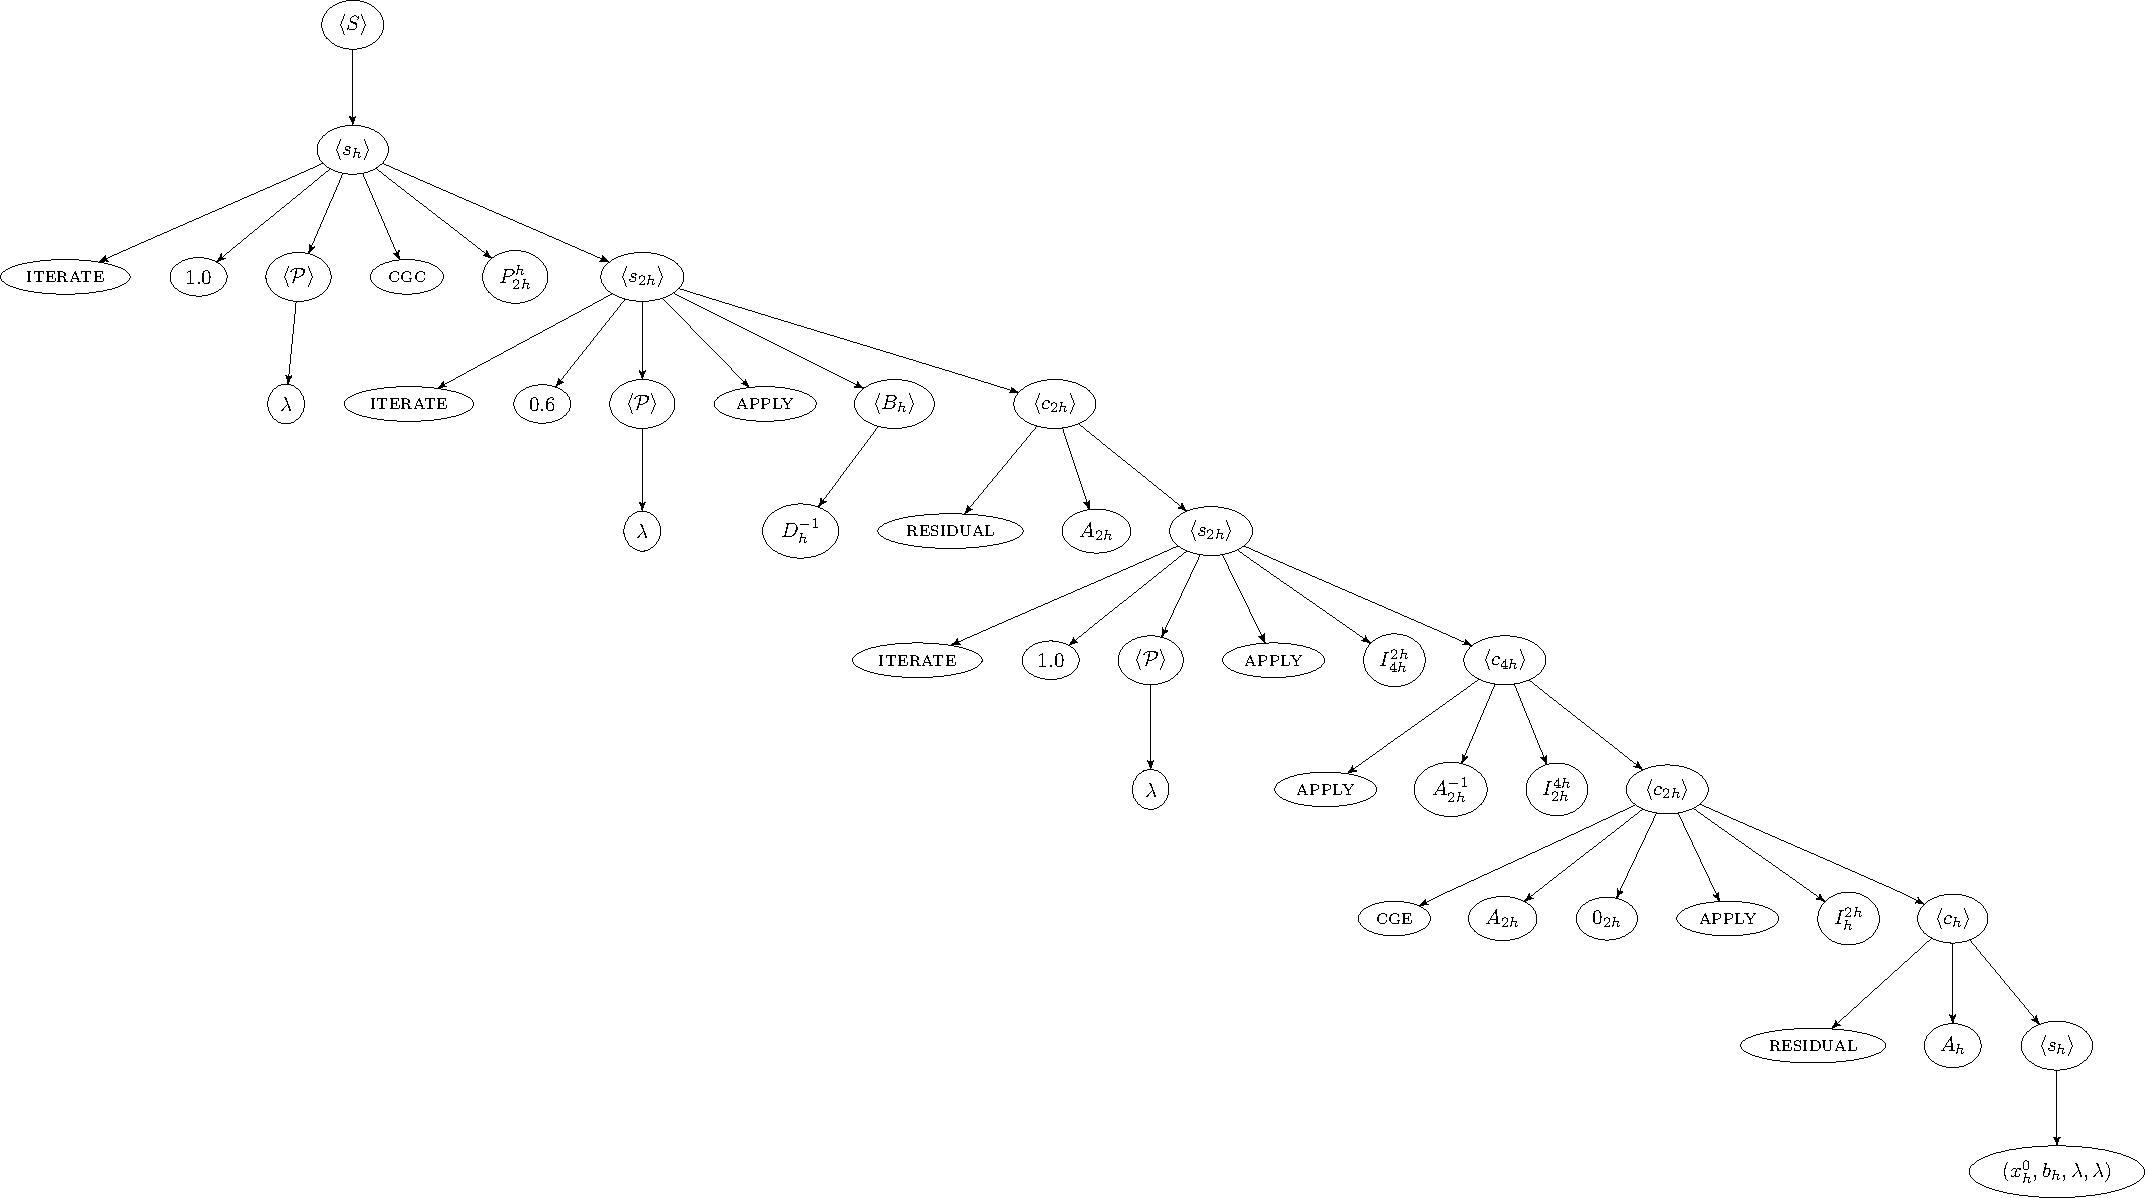
\includegraphics[width=\textwidth]{figures/trees/three_grid_method_grammar_tree.pdf}
	\caption{Grammar derivation tree for the three-grid method shown in Algorithm~\ref{alg:example-three-grid-method}.}
	\label{fig:example-three-grid-method-derivation-tree}
\end{figure}
Note that each inner node of the tree corresponds to a symbol that is contained in the set of variables $V$ of the grammar, as shown in Equation~\eqref{eq:multigrid-grammar-variables}, while all leaf nodes correspond to a terminal symbol.
As in the context of Table~\ref{table:multigrid-grammar} the application order of each function is well-defined, for the sake of simplicity, we have omitted all brackets in the tree.
%TODO evtl darauf eingehen, dass der CGS auf dem entsprechenden level spezifiziert sein muss
Until now we have been exclusively concerned with the problem of developing a formal representation for a multigrid method that is based on its algorithmic formulation, as for instance shown in Algorithm~\ref{alg:example-three-grid-method}, which can then be used to adapt each of its computational steps individually, granting us the possibility to apply the grammar-based program optimization techniques presented in Section~\ref{sec:gggp}.
However, in contrast to Figure~\ref{fig:example-three-grid-method-derivation-tree} where we have started with an algorithmic representation, within grammar-guided genetic programming (GGGP) a derivation tree is usually \emph{grown} by applying a sequence of productions in a randomly-chosen order, either to alter an already existing tree or to create a completely new one from scratch.
We, therefore, have to consider the task of obtaining a method's algorithmic formulation exclusively based on its representation as a derivation tree and with respect to the semantic evaluation rules that apply to each of its nodes.
As we have seen in Section~\ref{sec:multigrid-state-transitions} the application of each of the functions that are generated by our grammar returns a new state $S_H$ consisting of a tuple $\left( \tilde{x}_{H}, b_{H}, c_{H}, S_{H/2}\right)$, where $H$ is the discretization width on the current level.
Starting from the initial state tuple $\left(x_{h}^0, b_{h}, \lambda, \lambda\right)$ we can, therefore, apply the respective sequence of transition functions in a bottom-up manner, until we arrive at the final state $\left(\tilde{x}_{h}, b_{h}, \lambda, \lambda\right)$.
As we have shown in Figure~\ref{fig:example-tree-grid-method-states} the first component $\tilde{x}_{h}$ of this tuple then combines all steps of the corresponding multigrid method in a single expression
\begin{equation}
	\begin{split}
		\tilde{x}_h = \; & x_{h}^0 + I_{2h}^h ((x_{2h}^0 + I_{4h}^{2h} A_{4h}^{-1} I_{2h}^{4h} (I_{h}^{2h}(b_{h} - A_h x_{h}^0) - A_{2h} x_{2h}^0)) \\
		& + 0.6 \cdot D_{2h}^{-1} (I_{h}^{2h}(b_{h} - A_h x_{h}^0) - A_{2h} \\
		& \cdot (x_{2h}^0 + I_{4h}^{2h} A_{4h}^{-1} I_{2h}^{4h} (I_{h}^{2h}(b_{h} - A_h x_{h}^0) - A_{2h} x_{2h}^0)))).
		\label{eq:example-three-grid-method-expression}
	\end{split}
\end{equation}
While this expression contains all necessary information about the computational structure of the method, certain terms occur multiple times, which might lead the redundant computations.
We can, however, remove this redundancy by considering Equation~\eqref{eq:example-three-grid-method-expression} as a computational graph, where each node either corresponds to an arithmetic operation or to a predefined symbol, such as $x^0_h$, $b_h$ and $A_h$.
The resulting graph for Equation~\eqref{eq:example-three-grid-method-expression} is shown in Figure~\ref{fig:example-three-grid-method-computational-graph}.
\begin{figure}
	\centering
	\begin{subfigure}[b]{0.49\textwidth}
		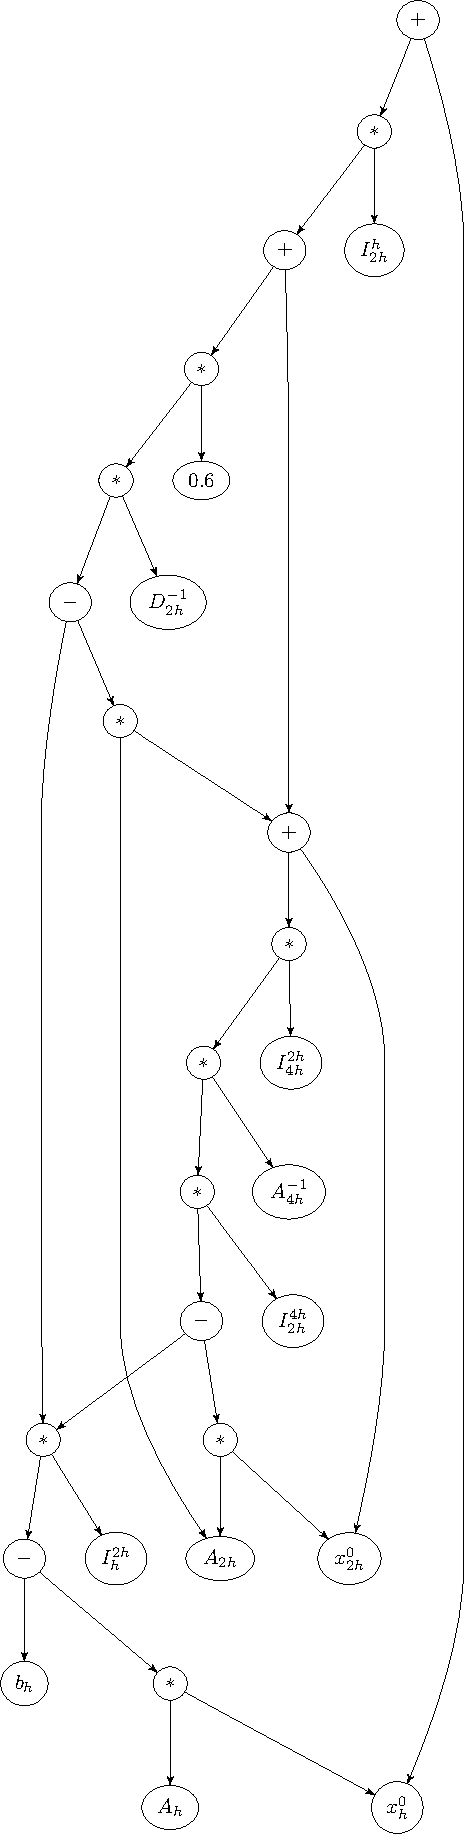
\includegraphics[scale=0.5]{figures/trees/three_grid_method_computational_graph.pdf}
		\caption{Original graph}
		\label{fig:example-three-grid-method-computational-graph-original}
	\end{subfigure}
	\centering
	\begin{subfigure}[b]{0.49\textwidth}
		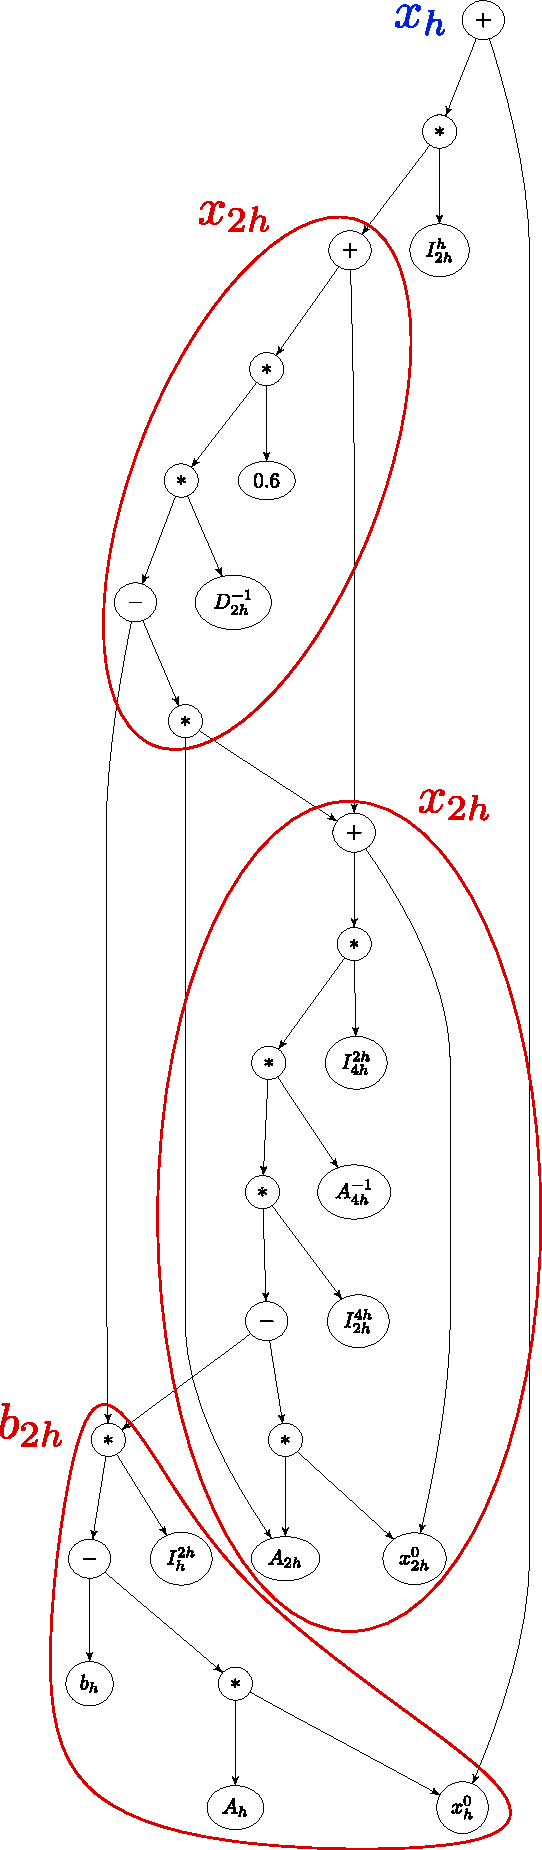
\includegraphics[scale=0.5]{figures/trees/three_grid_method_computational_graph_annotated.pdf}
		\caption{Annotated graph}
		\label{fig:example-three-grid-method-computational-graph-annotated}
	\end{subfigure}
	\caption{Computational graph for the three-grid method shown in Algorithm~\ref{alg:example-three-grid-method}.}
	\label{fig:example-three-grid-method-computational-graph}
\end{figure}
Again each node within this graph either corresponds to predefined symbol or an operation defined on vectors and matrices, whereby in case of the latter there exists a direct edge to each of the nodes that corresponds to one of its arguments.  
Therefore, whenever a certain node serves as an argument to more than one operations, multiple edges are directed towards it.
Based on this representation we can now define a redundancy-free sequence of computations that corresponds to the given multigrid method.
The most straightforward way to achieve this for a general graph is to simply introduce a temporary value for each non-leaf node of the graph.
However, note that each intermediate result in graph~\ref{fig:example-three-grid-method-computational-graph} that serves as an argument to multiple nodes either refers to a term representing the computation of an approximate solution or right-hand side on the respective level.
To verify this observation, consider again the three elementary multigrid operations listed in Definition~\ref{def:elementary-multigrid-operations}.
While a correction term is always discarded after its application, the current approximate solution is both needed in the construction of the current residual as well as whenever its value is updated, either through the application of smoothing or a coarse-grid correction.
Note that the same is true for the right-hand side, which is required whenever a new residual is constructed on a certain level.
This is illustrated in Figure~\ref{fig:example-three-grid-method-computational-graph-annotated}, where we have annotated all subgraph that correspond to the computation of an approximate solution or right-hand side.
Based on this graph we can now easily obtain an algorithmic representation for a multigrid solver while redundant computations are entirely avoided.
For this purpose, we first identify which node does not have any incoming edge and, hence, corresponds to the computation of the final approximate solution, which we have denoted as $\tilde{x}_h$ in Figure~\ref{fig:example-three-grid-method-computational-graph-annotated}.
The expression that needs to be assigned to this variable is then generated by recursively visiting the children of this node.
Note that since the graph is traversed starting from the last operation of the multigrid method, the algorithmic instructions are generated in reverse order. 
To avoid redundant computations, whenever a node is reached that either corresponds to an approximate solution or a right-hand side, we have to ensure that the respective subgraph is only generated once and assigned to a separate variable, which can then be referenced in all subsequent expressions.
The process of algorithm generations is continued until, in the end, only nodes without any outgoing edges have been reached.
For Figure~\ref{fig:example-three-grid-method-computational-graph-annotated} we, thus, obtain an algorithmic representation shown in Algorithm~\ref{alg:example-three-grid-method-generated} that is mathematically equivalent to the three-grid method formulated in Algorithm~\ref{alg:example-three-grid-method}, whereby the only difference is that certain intermediate expressions, such as the residual, are not assigned to a variable.
\begin{algorithm}
	\begin{algorithmic}[1]
		\State $ b_{2h} = I_{h}^{2h} \left(b_{h} - A_h x_{h}^0 \right)$
		\State $ \tilde{x}_{2h} = x^0_{2h} + I_{4h}^{2h} A_{4h}^{-1} I_{2h}^{4h} \left(b_{2h} - A_{2h} x^0_{2h}\right)$
		\State $ \tilde{x}_{2h} = \tilde{x}_{2h} + 0.6 \cdot D_{2h}^{-1} \left(b_{2h} - A_{2h} \tilde{x}_{2h}\right)$
		\State $\tilde{x}_{h} = \tilde{x}_{h}  + I_{2h}^h \tilde{x}_{2h}$
	\end{algorithmic}
	\caption{Three-grid multigrid method generated based on Figure~\ref{fig:example-three-grid-method-computational-graph-annotated}}
	\label{alg:example-three-grid-method-generated}
\end{algorithm}
Since we can apply the same approach to arbitrary computational graphs obtained from a derivation tree of our multigrid grammar, we obtain the following three-step approach for algorithm generation:
\begin{enumerate}
	\item Construct a multigrid method in form of its grammar derivation tree.
	\item Transform the derivation tree to a graph-based intermediate representation.
	\item Generate expressions for each approximate solution and right-hand side by means of recursive graph traversal.
\end{enumerate}
With the formulation of this approach, we have now outlined all necessary steps from the grammar-based generation of a multigrid method to its transformation to an algorithmic representation based on which can then apply these methods as numerical solvers.
However, we have not yet discussed in details how the individual steps of our approach, as described in this section, can be carried out in an automatic way on a modern computer.
In the remaining part of this thesis, we will, therefore, close these gaps by presenting our implementation of a grammar-guided multigrid optimization in form of the Python framework \emph{EvoStencils}, which is freely available as an open-source software library\footnote{EvoStencils: \url{https://github.com/jonas-schmitt/evostencils}}.
Since the EvoStencils framework builds substantially on the evolutionary optimization techniques presented in Section~\ref{sec:gggp}, it is important to consider first whether these algorithms are suitable for the given task or if a mere brute-force search is sufficient to identify the single best method among the set of possible ones for a given problem.
For this purpose, we aim to estimate the size of the search space that is created by the grammar formulated in Table~\ref{table:multigrid-grammar}, i.e. the number of different individuals that can be generated based on its productions.

\section{Search Space Estimation}
If we treat the grammar-based optimization of multigrid method as a search problem, the size of the search space spanned by the underlying grammar corresponds to the number of different methods that can be constructed based on its productions.
In practice, in case of a small search space it can be feasible to simply enumerate and evaluate all possible solutions of the given optimization problem, which has the advantage that the optimum is obtained in a deterministic manner while a heuristic search method, as those presented here in Section~\ref{sec:gggp}, is, in general, not guaranteed to find the same solution in each of its executions.
For this purpose, we consider the following simplified model calculation which acts as a lower bound of the size of the search space of a grammar-guided optimization of multigrid methods on a five-grid hierarchy, as defined by the grammar formulated in Table~\ref{table:multigrid-grammar}. 
As we have discussed in Section~\ref{sec:multigrid-methods} an effective multigrid method always employs a combination of smoothing and coarse-grid correction steps to efficiently reduce both the high and low-frequency components of the error.
While often in practice multiple smoothing steps are employed, the application of coarse-grid correction on a certain level without any smoothing is rarely used~\cite{trottenberg2000multigrid}.
To simplify the search space estimation, we, therefore, introduce the additional constraint that the total number of coarse-grid corrections is always equal or lower than the number of smoothing steps.
Furthermore, we enforce that restriction and prolongation can only be performed after smoothing, with the exception of the finest level, where we additionally allow restriction to be applied as a first operation.
As on finest level the original system is solved directly while smoothing is significantly more expensive than on subsequent levels, finding an optimal sequence of operations is of utmost importance for the efficiency of a multigrid method and we, hence, want to enforce fewer constraints on the order in which the individual operations are performed.
Consequently, using the symbols $S$, $R$ and $P$ for smoothing, restriction and prolongation, respectively, in each step of the method, depending on the level, only the following sequences of operations can be defined:
\begin{align*}
	S | RS | SR & \quad \text{for} \; l = l_{max} \\
	A^{-1} & \quad \text{for} \; l = l_{min} \\
	S | SR | SP & \quad \text{otherwise}.
\end{align*}
Therefore, with the exception of the coarsest level, where the only allowed operation is the application of the coarse-grid solver, the number of options for regarding the order of operations is always three.
However, since each step also includes the application of a smoother, we additionally have to choose a suitable method for this purpose.
Assuming the the number of available relaxation method is $n$, which includes different types of smoothers, partitionings and relaxation factors, this results in a total number of $3 \cdot n$ options in each step of the method. 
While none of these constraints is present in our original grammar shown in Table~\ref{table:multigrid-grammar}, they enable us to derive a simple closed-form expression which then acts as a lower bound for the actual size of the search space.
We can obtain such an expression in form of a finite sum of polynomials by considering the total number smoothing steps that are supposed to be performed within a multigrid method, whereby we know that for each step we need to choose from $3 \cdot n$ options independent from the level on which the operations are performed.
As a consequence, if our method incorporates $k$ smoothing steps, the total number of options is 
\begin{equation}
	N_{n,k} = (3 n)^k
	\label{eq:simplified-number-of-options}
\end{equation}
We can illustrate this observation by considering the corresponding decision tree, which is shown in Figure~\ref{fig:decision-tree} for $n = 2$.
\begin{figure}
	\centering
	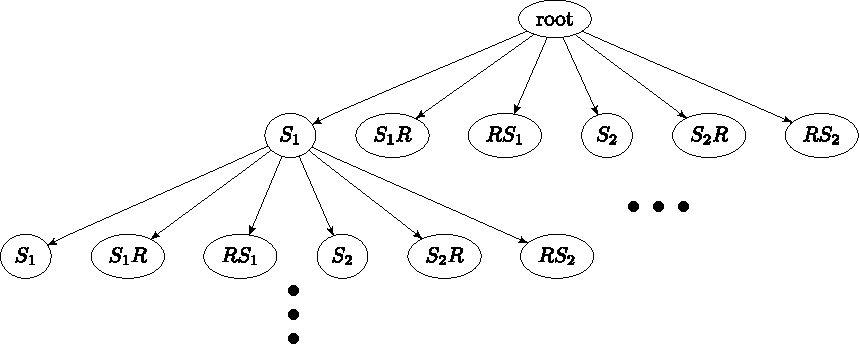
\includegraphics[width=\textwidth]{figures/trees/decision_tree_annotated.pdf}
	\caption{Simplified decision tree - Each node has the same number of children.}
	\label{fig:decision-tree}
\end{figure}
Each node in this tree corresponds to a particular choice from the available set of options.
Since each step within our simplified decision model includes the application of either $S_1$ or $S_2$ as a smoother which can then optionally be complemented with restriction or prolongation, the depth of the tree is equal to the total number of smoothing steps $k$ applied within the corresponding multigrid method.
Consequently, each leaf of the tree corresponds to a different multigrid method, and the total number of leaves is thus equal to $N_{2,k} = 6^k$.
However, since the optimal amount of smoothing depends on the properties of the linear system that we aim to solve and a varying total number of smoothing steps should be considered for each problem.
Now note that each decision tree that corresponds to a certain number of smoothing steps $k$ contains all those with less smoothing steps as a subtree, whereby each subtree is obtained by performing a top-down breadth-first traversal until the depth of the tree coincides with the respective number of smoothing steps.
Therefore, the total number of different multigrid methods with at least $k_{min}$ but at most $k_{max}$ smoothing steps is equal to the total number of leaf nodes of all subtrees of a decision tree of depth $k_{max}$ that have at least depth $k_{min}$.
As we have already seen the number of leaf nodes of a decision tree with depth is given by Equation~\ref{eq:simplified-number-of-options}.
Hence, the total number of different multigrid methods that employ between $k_{min}$ and $k_{max}$ smoothing steps is given by the finite sum
\begin{equation}
	N(n, k_{min}, k_{max}) = \sum_{k = k_{min}}^{k_{max}} N_{n,k} = \sum_{k = k_{min}}^{k_{max}} (3 n)^k.
	\label{eq:search-space-estimation}
\end{equation}
We can now finally utilize this formula to obtain an estimated lower bound for the total number of different five-grid method that can be constructed with the grammar formulated in Table~\ref{table:multigrid-grammar}.
For this purpose, we need to choose a reasonable interval for the minimum and maximum total number of smoothing steps of our method.
In Algorithm~\ref{alg:multigrid-cycle} the total number of smoothing steps per level depends on the parameters $\nu_1$, $\nu_2$ and $\gamma$, which specify the number of pre-smoothing steps, post-smoothing steps and recursive descents per level, respectively.
Therefore, the total number of smoothing steps is given by
\begin{equation*}
	\sum_{k = 0}^{n_c - 1} \gamma^k (\nu_1 + \nu_2),
\end{equation*}
where $n_c$ is the number of coarsening steps.
%TODO only true for W-cycle, fix formula!
Now let us consider how different choices of $\nu_1$, $\nu_2$ and $\gamma$ lead to a different number of total smoothing steps for a five-grid method ($n_c = 4$):
\begin{itemize}
	\item $V(1,0)$: $\gamma = 1, \nu_1 = 1, \nu_2 = 0 \Rightarrow 4 \; \text{smoothing steps}$
	\item $V(3,3)$: $\gamma = 1, \nu_1 = 3, \nu_2 = 3 \Rightarrow 24 \; \text{smoothing steps}$
	\item $W(1,0)$: $\gamma = 2, \nu_1 = 1, \nu_2 = 0 \Rightarrow 15 \; \text{smoothing steps}$
	\item $W(1,1)$: $\gamma = 2, \nu_1 = 1, \nu_2 = 0 \Rightarrow 30 \; \text{smoothing steps}$
	\item $W(3,3)$: $\gamma = 2, \nu_1 = 3, \nu_2 = 3 \Rightarrow 90 \; \text{smoothing steps}$
\end{itemize}
Setting $k_{min} = 4$ and $k_{max} = 30$ as an upper limit for the number of smoothing steps in Equation~\ref{eq:search-space-estimation}, hence, represents a reasonable compromise, as it allows us to generate multigrid methods that perform a similar amount of smoothing steps as the majority of commonly used $V$-cycles while at the same methods comparable to less expensive $W$-cycle variants can be also obtained.
Finally, the only remaining parameter is the number of different relaxation methods from which we can choose in each smoothing step.
To obtain a conservative estimate for a lower bound of the search space size we set $n = 2$, which means that in each step we only have to choose from two alternatives, for example the Jacobi and red-black Gauss-Seidel method.
By utilizing Equation~\eqref{eq:search-space-estimation} we, therefore, obtain 
\begin{equation*}
	N(2, 4, 30) = \sum_{k = 4}^{30} 6^k \approx 2.65 \cdot 10^{24}
\end{equation*}
as an estimated lower bound for the search space spanned by the grammar formulated in Table~\ref{table:multigrid-grammar}.
If we now assume that a modern multi-core CPU is capable of evaluating each multigrid method in an average time of one millisecond,
even a supercomputer consisting of one trillion ($10^{12}$) such processors would require more than 8 years to evaluate all methods that are contained in this search space.
Furthermore, in practice it is usually beneficial to consider a higher number of different smoothers and relaxation factors, which results in an even larger search space.
As a consequence, while a pure brute-force-approach that aims to evaluate all possible multigrid methods may be feasible for the constrained parameter space that results from the classical formulation in Algorithm~\ref{alg:multigrid-cycle}, a grammar-based optimization requires the utilization of search strategies, such as grammar-guided genetic programming (GGGP) as it has been presented in Section~\ref{sec:gggp}.
\paragraph{Final Remarks}
In the remainder of this thesis we will describe how GGGP can be applied within \emph{EvoStencils}, our implementation of a grammar-guided optimization of multigrid methods in the Python programming language, which is based on the formal framework presented in this chapter.
We will, furthermore, demonstrate EvoStencils' effectiveness by evolving efficient multigrid methods for a number of different partial differential equations (PDEs).
In the following we, therefore, assume the reader to be familiar with Python, due to its widespread use in both academia and industry.
If this should not be the case the reader is advised to consult one of the many available resources for learning Python\footnote{Python:~\url{https://www.python.org/doc/}}.
Along with this we also assume basic knowledge about programming and parallelization techniques for recent multiprocessor and cluster systems, of which an overview can be found in~\cite{sterling2017high,hager2010introduction}.
%Furthermore, while hardware-specific code optimization is not a focus of this thesis, the reader should have some basic understanding about the architectural features of recent multiprocessor systems and supercomputers.
%Along with this, we also assume a familiarity with programming techniques and tools for performing a shared and distributed memory parallelization on these systems, such as OpenMP\footnote{OpenMP:~\url{https://www.openmp.org/}} and MPI\footnote{MPI:~\url{https://www.mpi-forum.org/}}. 
%\begin{figure}
%	\captionsetup{justification=centering}
%	\begin{subfigure}{0.1\textwidth}
%		\begin{tikzpicture}
%			\node   (h) at (-0.75, 4){$h$};
%			\node   (2h) at (-0.75, 3){$2h$};
%			\node   (4h) at (-0.75, 2){$4h$};
%			\node   (8h) at (-0.75, 1){$8h$};
%			\node   (16h) at (-0.75, 0){$8h$};
%		\end{tikzpicture}
%	\end{subfigure}
%	\begin{subfigure}{0.9\textwidth}
%		\begin{tikzpicture}
%			\node	(a) at (0,4) [draw, circle,fill=blue,scale=0.8] {};
%			\node	(b) at (0.5,3) [draw, circle, fill=blue, scale=0.8] {};
%			\node	(c) at (1,2) [draw, circle, fill=blue, scale=0.8] {};
%			\node	(d) at (1.5,1) [draw, circle, fill=blue, scale=0.8] {};
%			\node	(e) at (2,0) [draw, circle, ,fill=black, scale=0.8] {};
%			\node	(f) at (2.5,1) [draw, circle,scale=0.8] {};
%			\node	(g) at (3,2) [draw, circle,scale=0.8] {};
%			\node	(h) at (3.5,3) [draw, circle, scale=0.8] {};
%			\node	(i) at (4,4) [draw, circle,scale=0.8] {};
%			\draw 
%			(a) edge[->] (b) 
%			(b) edge[->] (c)
%			(c) edge[->] (d)
%			(d) edge[->] (e)   
%			(e) edge[->] (f)
%			(f) edge[->] (g)
%			(g) edge[->] (h)
%			(h) edge[->] (i)
%			;
%		\end{tikzpicture}
%	\end{subfigure}
%	
%	\caption{Five-grid cycle with $\nu_1 = 1$ and $\nu_2 = 0$. Smoothing is only performed in the steps corresponding to blue-colored nodes.}
%	\label{fig:five-grid-V-cycle}
%\end{figure}

